
%% bare_conf.tex
%% V1.3
%% 2007/01/11
%% by Michael Shell
%% See:
%% http://www.michaelshell.org/
%% for current contact information.
%%
%% This is a skeleton file demonstrating the use of IEEEtran.cls
%% (requires IEEEtran.cls version 1.7 or later) with an IEEE conference paper.
%%
%% Support sites:
%% http://www.michaelshell.org/tex/ieeetran/
%% http://www.ctan.org/tex-archive/macros/latex/contrib/IEEEtran/
%% and
%% http://www.ieee.org/

%%*************************************************************************
%% Legal Notice:
%% This code is offered as-is without any warranty either expressed or
%% implied; without even the implied warranty of MERCHANTABILITY or
%% FITNESS FOR A PARTICULAR PURPOSE! 
%% User assumes all risk.
%% In no event shall IEEE or any contributor to this code be liable for
%% any damages or losses, including, but not limited to, incidental,
%% consequential, or any other damages, resulting from the use or misuse
%% of any information contained here.
%%
%% All comments are the opinions of their respective authors and are not
%% necessarily endorsed by the IEEE.
%%
%% This work is distributed under the LaTeX Project Public License (LPPL)
%% ( http://www.latex-project.org/ ) version 1.3, and may be freely used,
%% distributed and modified. A copy of the LPPL, version 1.3, is included
%% in the base LaTeX documentation of all distributions of LaTeX released
%% 2003/12/01 or later.
%% Retain all contribution notices and credits.
%% ** Modified files should be clearly indicated as such, including  **
%% ** renaming them and changing author support contact information. **
%%
%% File list of work: IEEEtran.cls, IEEEtran_HOWTO.pdf, bare_adv.tex,
%%                    bare_conf.tex, bare_jrnl.tex, bare_jrnl_compsoc.tex
%%*************************************************************************

% *** Authors should verify (and, if needed, correct) their LaTeX system  ***
% *** with the testflow diagnostic prior to trusting their LaTeX platform ***
% *** with production work. IEEE's font choices can trigger bugs that do  ***
% *** not appear when using other class files.                            ***
% The testflow support page is at:
% http://www.michaelshell.org/tex/testflow/



% Note that the a4paper option is mainly intended so that authors in
% countries using A4 can easily print to A4 and see how their papers will
% look in print - the typesetting of the document will not typically be
% affected with changes in paper size (but the bottom and side margins will).
% Use the testflow package mentioned above to verify correct handling of
% both paper sizes by the user's LaTeX system.
%
% Also note that the "draftcls" or "draftclsnofoot", not "draft", option
% should be used if it is desired that the figures are to be displayed in
% draft mode.
%
\documentclass[conference]{IEEEtran}
% Add the compsoc option for Computer Society conferences.
%
% If IEEEtran.cls has not been installed into the LaTeX system files,
% manually specify the path to it like:
% \documentclass[conference]{../sty/IEEEtran}

%\IEEEoverridecommandlockouts

%\IEEEpubid{978-1-4799-0898-1/13/\$31.00~\copyright~2013 IEEE}
%\IEEEpubid{\makebox[\columnwidth]{\hfill 978-1-4799-0898-1/13/\$31.00~\copyright~2013 IEEE}%
%\hspace{\columnsep}\makebox[\columnwidth]{}}


% Some very useful LaTeX packages include:
% (uncomment the ones you want to load)


% *** MISC UTILITY PACKAGES ***
%
\usepackage{ifpdf}
% Heiko Oberdiek's ifpdf.sty is very useful if you need conditional
% compilation based on whether the output is pdf or dvi.
% usage:
% \ifpdf
%   % pdf code
% \else
%   % dvi code
% \fi
% The latest version of ifpdf.sty can be obtained from:
% http://www.ctan.org/tex-archive/macros/latex/contrib/oberdiek/
% Also, note that IEEEtran.cls V1.7 and later provides a builtin
% \ifCLASSINFOpdf conditional that works the same way.
% When switching from latex to pdflatex and vice-versa, the compiler may
% have to be run twice to clear warning/error messages.






% *** CITATION PACKAGES ***
%
\usepackage{cite}
% cite.sty was written by Donald Arseneau
% V1.6 and later of IEEEtran pre-defines the format of the cite.sty package
% \cite{} output to follow that of IEEE. Loading the cite package will
% result in citation numbers being automatically sorted and properly
% "compressed/ranged". e.g., [1], [9], [2], [7], [5], [6] without using
% cite.sty will become [1], [2], [5]--[7], [9] using cite.sty. cite.sty's
% \cite will automatically add leading space, if needed. Use cite.sty's
% noadjust option (cite.sty V3.8 and later) if you want to turn this off.
% cite.sty is already installed on most LaTeX systems. Be sure and use
% version 4.0 (2003-05-27) and later if using hyperref.sty. cite.sty does
% not currently provide for hyperlinked citations.
% The latest version can be obtained at:
% http://www.ctan.org/tex-archive/macros/latex/contrib/cite/
% The documentation is contained in the cite.sty file itself.






% *** GRAPHICS RELATED PACKAGES ***
%
\ifCLASSINFOpdf
  \usepackage[pdftex]{graphicx}
  % declare the path(s) where your graphic files are
  \graphicspath{{./pics/}}
  % and their extensions so you won't have to specify these with
  % every instance of \includegraphics
  \DeclareGraphicsExtensions{.pdf,.jpeg,.jpg,.png}
\else
  % or other class option (dvipsone, dvipdf, if not using dvips). graphicx
  % will default to the driver specified in the system graphics.cfg if no
  % driver is specified.
  \usepackage[dvips]{graphicx}
  % declare the path(s) where your graphic files are
  \graphicspath{{./pics/}}
  % and their extensions so you won't have to specify these with
  % every instance of \includegraphics
  \DeclareGraphicsExtensions{.eps}
\fi
% graphicx was written by David Carlisle and Sebastian Rahtz. It is
% required if you want graphics, photos, etc. graphicx.sty is already
% installed on most LaTeX systems. The latest version and documentation can
% be obtained at: 
% http://www.ctan.org/tex-archive/macros/latex/required/graphics/
% Another good source of documentation is "Using Imported Graphics in
% LaTeX2e" by Keith Reckdahl which can be found as epslatex.ps or
% epslatex.pdf at: http://www.ctan.org/tex-archive/info/
%
% latex, and pdflatex in dvi mode, support graphics in encapsulated
% postscript (.eps) format. pdflatex in pdf mode supports graphics
% in .pdf, .jpeg, .png and .mps (metapost) formats. Users should ensure
% that all non-photo figures use a vector format (.eps, .pdf, .mps) and
% not a bitmapped formats (.jpeg, .png). IEEE frowns on bitmapped formats
% which can result in "jaggedy"/blurry rendering of lines and letters as
% well as large increases in file sizes.
%
% You can find documentation about the pdfTeX application at:
% http://www.tug.org/applications/pdftex





% *** MATH PACKAGES ***
%
%\usepackage[cmex10]{amsmath}
% A popular package from the American Mathematical Society that provides
% many useful and powerful commands for dealing with mathematics. If using
% it, be sure to load this package with the cmex10 option to ensure that
% only type 1 fonts will utilized at all point sizes. Without this option,
% it is possible that some math symbols, particularly those within
% footnotes, will be rendered in bitmap form which will result in a
% document that can not be IEEE Xplore compliant!
%
% Also, note that the amsmath package sets \interdisplaylinepenalty to 10000
% thus preventing page breaks from occurring within multiline equations. Use:
%\interdisplaylinepenalty=2500
% after loading amsmath to restore such page breaks as IEEEtran.cls normally
% does. amsmath.sty is already installed on most LaTeX systems. The latest
% version and documentation can be obtained at:
% http://www.ctan.org/tex-archive/macros/latex/required/amslatex/math/





% *** SPECIALIZED LIST PACKAGES ***
%
%\usepackage{algorithmic}
% algorithmic.sty was written by Peter Williams and Rogerio Brito.
% This package provides an algorithmic environment fo describing algorithms.
% You can use the algorithmic environment in-text or within a figure
% environment to provide for a floating algorithm. Do NOT use the algorithm
% floating environment provided by algorithm.sty (by the same authors) or
% algorithm2e.sty (by Christophe Fiorio) as IEEE does not use dedicated
% algorithm float types and packages that provide these will not provide
% correct IEEE style captions. The latest version and documentation of
% algorithmic.sty can be obtained at:
% http://www.ctan.org/tex-archive/macros/latex/contrib/algorithms/
% There is also a support site at:
% http://algorithms.berlios.de/index.html
% Also of interest may be the (relatively newer and more customizable)
% algorithmicx.sty package by Szasz Janos:
% http://www.ctan.org/tex-archive/macros/latex/contrib/algorithmicx/




% *** ALIGNMENT PACKAGES ***
%
%\usepackage{array}
% Frank Mittelbach's and David Carlisle's array.sty patches and improves
% the standard LaTeX2e array and tabular environments to provide better
% appearance and additional user controls. As the default LaTeX2e table
% generation code is lacking to the point of almost being broken with
% respect to the quality of the end results, all users are strongly
% advised to use an enhanced (at the very least that provided by array.sty)
% set of table tools. array.sty is already installed on most systems. The
% latest version and documentation can be obtained at:
% http://www.ctan.org/tex-archive/macros/latex/required/tools/


%\usepackage{mdwmath}
%\usepackage{mdwtab}
% Also highly recommended is Mark Wooding's extremely powerful MDW tools,
% especially mdwmath.sty and mdwtab.sty which are used to format equations
% and tables, respectively. The MDWtools set is already installed on most
% LaTeX systems. The lastest version and documentation is available at:
% http://www.ctan.org/tex-archive/macros/latex/contrib/mdwtools/


% IEEEtran contains the IEEEeqnarray family of commands that can be used to
% generate multiline equations as well as matrices, tables, etc., of high
% quality.


%\usepackage{eqparbox}
% Also of notable interest is Scott Pakin's eqparbox package for creating
% (automatically sized) equal width boxes - aka "natural width parboxes".
% Available at:
% http://www.ctan.org/tex-archive/macros/latex/contrib/eqparbox/





% *** SUBFIGURE PACKAGES ***
\usepackage[labelfont=bf,labelsep=space,list=true]{subcaption}
%\usepackage[tight,footnotesize]{subfigure}
% subfigure.sty was written by Steven Douglas Cochran. This package makes it
% easy to put subfigures in your figures. e.g., "Figure 1a and 1b". For IEEE
% work, it is a good idea to load it with the tight package option to reduce
% the amount of white space around the subfigures. subfigure.sty is already
% installed on most LaTeX systems. The latest version and documentation can
% be obtained at:
% http://www.ctan.org/tex-archive/obsolete/macros/latex/contrib/subfigure/
% subfigure.sty has been superceeded by subfig.sty.



%\usepackage[caption=false]{caption}
%\usepackage[font=footnotesize]{subfig}
% subfig.sty, also written by Steven Douglas Cochran, is the modern
% replacement for subfigure.sty. However, subfig.sty requires and
% automatically loads Axel Sommerfeldt's caption.sty which will override
% IEEEtran.cls handling of captions and this will result in nonIEEE style
% figure/table captions. To prevent this problem, be sure and preload
% caption.sty with its "caption=false" package option. This is will preserve
% IEEEtran.cls handing of captions. Version 1.3 (2005/06/28) and later 
% (recommended due to many improvements over 1.2) of subfig.sty supports
% the caption=false option directly:
%\usepackage[caption=false,font=footnotesize]{subfig}
%
% The latest version and documentation can be obtained at:
% http://www.ctan.org/tex-archive/macros/latex/contrib/subfig/
% The latest version and documentation of caption.sty can be obtained at:
% http://www.ctan.org/tex-archive/macros/latex/contrib/caption/




% *** FLOAT PACKAGES ***
%
%\usepackage{fixltx2e}
% fixltx2e, the successor to the earlier fix2col.sty, was written by
% Frank Mittelbach and David Carlisle. This package corrects a few problems
% in the LaTeX2e kernel, the most notable of which is that in current
% LaTeX2e releases, the ordering of single and double column floats is not
% guaranteed to be preserved. Thus, an unpatched LaTeX2e can allow a
% single column figure to be placed prior to an earlier double column
% figure. The latest version and documentation can be found at:
% http://www.ctan.org/tex-archive/macros/latex/base/



%\usepackage{stfloats}
% stfloats.sty was written by Sigitas Tolusis. This package gives LaTeX2e
% the ability to do double column floats at the bottom of the page as well
% as the top. (e.g., "\begin{figure*}[!b]" is not normally possible in
% LaTeX2e). It also provides a command:
%\fnbelowfloat
% to enable the placement of footnotes below bottom floats (the standard
% LaTeX2e kernel puts them above bottom floats). This is an invasive package
% which rewrites many portions of the LaTeX2e float routines. It may not work
% with other packages that modify the LaTeX2e float routines. The latest
% version and documentation can be obtained at:
% http://www.ctan.org/tex-archive/macros/latex/contrib/sttools/
% Documentation is contained in the stfloats.sty comments as well as in the
% presfull.pdf file. Do not use the stfloats baselinefloat ability as IEEE
% does not allow \baselineskip to stretch. Authors submitting work to the
% IEEE should note that IEEE rarely uses double column equations and
% that authors should try to avoid such use. Do not be tempted to use the
% cuted.sty or midfloat.sty packages (also by Sigitas Tolusis) as IEEE does
% not format its papers in such ways.





% *** PDF, URL AND HYPERLINK PACKAGES ***
%
\usepackage{url}
% url.sty was written by Donald Arseneau. It provides better support for
% handling and breaking URLs. url.sty is already installed on most LaTeX
% systems. The latest version can be obtained at:
% http://www.ctan.org/tex-archive/macros/latex/contrib/misc/
% Read the url.sty source comments for usage information. Basically,
% \url{my_url_here}.





% *** Do not adjust lengths that control margins, column widths, etc. ***
% *** Do not use packages that alter fonts (such as pslatex).         ***
% There should be no need to do such things with IEEEtran.cls V1.6 and later.
% (Unless specifically asked to do so by the journal or conference you plan
% to submit to, of course. )


% correct bad hyphenation here
\hyphenation{op-tical net-works semi-conduc-tor}

%-------------------------------------------------------------------------
% Our Stuff
%-------------------------------------------------------------------------
% For transparency (do not remove)
\pdfpageattr{/Group <</S /Transparency /I true /CS /DeviceRGB>>}

%% Spacing adjustments
\usepackage{textcomp} % Must be loaded to prevent conflict microtype/siunitx
\usepackage{microtype}

% Nicer tabs
\usepackage{booktabs}

% TikZ
\usepackage{tikz}
\usepackage{gnuplot-lua-tikz}
\usetikzlibrary{tikzmark, calc, patterns, shapes, positioning,arrows,
  decorations.pathmorphing, decorations.pathreplacing, decorations.text,
  math, trees, shadows}

% Additional colors
\usepackage{xcolor}
%\colorlet{paperblue}{-red!75!green!50} %206080 ?
%\definecolor{paperblue}{RGB}{0,96,173}
\colorlet{paperblue}{-red!75!green!50}
%\colorlet{paperblue}{black}

% Tikz macros
\tikzset{%
  highlight/.style={rectangle,rounded corners,draw,thick}
}
\newcommand{\tablearrowright}[4]{%
  \tikz[overlay,remember picture]{
  \draw ($(pic cs:#1) + (5pt,4pt)$) edge[bend right=45,-stealth]
        ($(pic cs:#2) + (5pt,4pt)$)
        node [highlight,right,xshift=5pt,yshift=7pt,#4] {#3};}
}
\newcommand{\tablearrowleft}[4]{%
  \tikz[overlay,remember picture]{
  \draw ($(pic cs:#1) + (5pt,2pt)$) edge[bend left=45,-stealth]
        ($(pic cs:#2) + (5pt,2pt)$)
        node [highlight,right,xshift=5pt,yshift=-7pt,#4] {#3};}
}

% SI units
\usepackage[binary-units]{siunitx}
\sisetup{per-mode = symbol}
\providecommand{\gbps}[1]{\SI{#1}{\giga\byte\per\second}}
\providecommand{\mbps}[1]{\SI{#1}{\mega\byte\per\second}}
\providecommand{\gb}[1]{\SI{#1}{\giga\byte}}
\providecommand{\mb}[1]{\SI{#1}{\mega\byte}}
\providecommand{\kb}[1]{\SI{#1}{\kilo\byte}}
\providecommand{\ms}[1]{\SI{#1}{\milli\second}}

% Code snippets
\usepackage{listings}
\def\lstsetc{\lstset{language=C,
%  numbers=left,
%  xleftmargin=2.2em,
  xleftmargin=1.8em,
  framexleftmargin=0.2em,
  numberstyle=\tiny\color{gray},
  stepnumber=1,
  showspaces=false, 
  showstringspaces=false,
  breaklines=true,
  basicstyle=\footnotesize\ttfamily,
  stringstyle=\itshape,
  commentstyle=\itshape\bfseries,
  frame=leftline,
  morekeywords={main, size_t, malloc, free, write, H5Screate_simple},
  morekeywords={[2]H5S_UNLIMITED},
  keywordstyle={[2]\color{gray}\bfseries}
  }
}

\begin{document}

%
% paper title
% can use linebreaks \\ within to get better formatting as desired
\title{Extending HDF5 Datasets: Enhancements to the Chunk Indexing Methods}

% author names and affiliations
% use a multiple column layout for up to three different
% affiliations
%\author{\IEEEauthorblockN{Jerome Soumagne}
%\IEEEauthorblockA{The HDF Group\\
%Champaign, IL 61820\\
%Email: jsoumagne@hdfgroup.org}
%\and
%\IEEEauthorblockN{Dries Kimpe}
%\IEEEauthorblockA{Argonne National Laboratory\\
%Argonne, IL 60439\\
%Email: dkimpe@mcs.anl.gov}
%\and
%\IEEEauthorblockN{Mohamad Chaarawi}
%\IEEEauthorblockA{The HDF Group\\
%Champaign, IL 61820\\
%Email: chaarawi@hdfgroup.org}
%\and
%\IEEEauthorblockN{Quincey Koziol}
%\IEEEauthorblockA{The HDF Group\\
%Champaign, IL 61820\\
%Email: koziol@hdfgroup.org}
%}

% conference papers do not typically use \thanks and this command
% is locked out in conference mode. If really needed, such as for
% the acknowledgment of grants, issue a \IEEEoverridecommandlockouts
% after \documentclass

% for over three affiliations, or if they all won't fit within the width
% of the page, use this alternative format:
% 
\author{\IEEEauthorblockN{Vailin Choi\IEEEauthorrefmark{1},
Jerome Soumagne\IEEEauthorrefmark{1}
Quincey Koziol\IEEEauthorrefmark{1}
}
\IEEEauthorblockA{\IEEEauthorrefmark{1}The HDF Group\\
Champaign, IL 61820}
}




% use for special paper notices
%\IEEEspecialpapernotice{(Invited Paper)}




% make the title area
\maketitle


\begin{abstract}

The HDF5 library requires the use of chunking when defining extendable datasets. Chunking makes it possible to extend datasets efficiently without having to reorganize contiguous storage excessively. However, to retrieve elements in the datasets that are stored in chunked form, the chunk containing those elements must be located and accessed. Therefore, the library must define and use efficient indexing methods for the retrieval of those chunks. We present in this paper the indexing methods that are being used, as well as some of the enhancements made to improve performance of these methods.

\end{abstract}
% IEEEtran.cls defaults to using nonbold math in the Abstract.
% This preserves the distinction between vectors and scalars. However,
% if the conference you are submitting to favors bold math in the abstract,
% then you can use LaTeX's standard command \boldmath at the very start
% of the abstract to achieve this. Many IEEE journals/conferences frown on
% math in the abstract anyway.

% no keywords




% For peer review papers, you can put extra information on the cover
% page as needed:
% \ifCLASSOPTIONpeerreview
% \begin{center} \bfseries EDICS Category: 3-BBND \end{center}
% \fi
%
% For peerreview papers, this IEEEtran command inserts a page break and
% creates the second title. It will be ignored for other modes.
\IEEEpeerreviewmaketitle

% Say that there are 2 ulimited dimensions for XY extended

\section{Introduction}

The HDF5 library~\cite{Folk2011}\cite{Folk1999} provides users with a high degree of flexibility for data
management---users may define and organize data into different groups and
datasets and build an hierarchical tree of data. Datasets may be contiguously 
mapped from the application memory to a file, or stored in more complex 
patterns to ease further access and analysis of the data. One option that
is commonly used is to create and define a dataset as \textit{extendable},
in order to easily append new values to it.
An HDF5 dataset is extendable when the maximum dimension sizes of its 
dataspace are greater than the current dimension sizes, with the maximum dimension 
size being specified as \textit{fixed} size or \textit{unlimited} size.

When defining an extendable dataset, the HDF5 library requires the dataset
to be partitioned into fixed-size multi-dimensional chunks---this operation, 
illustrated in figure~\ref{fig:hdf5_dataset}, is called \textit{chunking}.
Chunking makes it possible to extend datasets efficiently without having to
reorganize contiguous storage excessively. To retrieve elements in the
datasets that are stored in chunked form, the chunk containing those
elements must be located and accessed. Several structures can be used
to achieve that and the locations of chunks for a dataset have originally 
been stored in a B-tree data structure. This structure maps the index of the chunk to 
the file offset where the chunk's elements are stored. However, depending
on the use case and in particular for extendable datasets, it presents some
drawbacks, which are addressed in this paper.

This paper is organized as follows. 
Section~\ref{sec:architecture} presents the 
current indexing method used within the library for chunking as well as 
modifications that were made to improve performance when a dataset is 
being extended. Section~\ref{sec:evaluation} presents performance evaluation 
results. In Section~\ref{sec:related_work} we discuss related work before
presenting conclusions and future research directions in Section~\ref{sec:conclusion}.

\begin{figure}
\begin{subfigure}[b]{.49\linewidth}
\centering
\def\drawdataset#1#2#3#4{%
\begin{scope}[#1]
\tikzmath{
  if #3 >= 0 then {
  for \y in {1,...,#2}{
    {
    \pgfmathparse{#3 + #2 - \y}
    \pgfmathtruncatemacro{\ylabel}{\pgfmathresult}
    \path[fill=white,postaction={decorate},
      decoration={text along path,text={|\small|~\ylabel~||},text align=center,raise=4pt}
      ] (0,\y) -- ++(1,0);
    };
  };
  };
  if #4 >= 0 then {
  for \x in {1,...,#2}{
    {
    \pgfmathparse{#4 + \x - 1}
    \pgfmathtruncatemacro{\xlabel}{\pgfmathresult}
    \path[fill=white,postaction={decorate},
      decoration={text along path,text={|\small|~\xlabel~||},text align=center,raise=4pt}
      ] (\x,#2 + 1) -- ++(1,0);
    };
  };
  };
  for \y in {1,...,#2}{
    for \x in {1,...,#2}{
      {
      \path[fill=white,draw=gray] (\x,\y) rectangle ++(1,1);
      };
    };
  };
}
\path[draw=paperblue,thick] (1,1) rectangle (#2 + 1,#2 + 1);
\end{scope}
}



\begin{tikzpicture}

\drawdataset{scale=0.5}{6}{0}{0}

\end{tikzpicture}

\caption{Contiguous.}
\label{fig:contiguous}
\end{subfigure}%
\hfill
\begin{subfigure}[b]{.49\linewidth}
\centering
\def\drawdataset#1#2#3#4{%
\begin{scope}[#1]
\tikzmath{
  if #3 >= 0 then {
  for \y in {1,...,#2}{
    {
    \pgfmathparse{#3 + #2 - \y}
    \pgfmathtruncatemacro{\ylabel}{\pgfmathresult}
    \path[fill=white,postaction={decorate},
      decoration={text along path,text={|\small|~\ylabel~||},text align=center,raise=4pt}
      ] (0,\y) -- ++(1,0);
    };
  };
  };
  if #4 >= 0 then {
  for \x in {1,...,#2}{
    {
    \pgfmathparse{#4 + \x - 1}
    \pgfmathtruncatemacro{\xlabel}{\pgfmathresult}
    \path[fill=white,postaction={decorate},
      decoration={text along path,text={|\small|~\xlabel~||},text align=center,raise=4pt}
      ] (\x,#2 + 1) -- ++(1,0);
    };
  };
  };
  for \y in {1,...,#2}{
    for \x in {1,...,#2}{
      {
      \path[fill=white,draw=gray] (\x,\y) rectangle ++(1,1);
      };
    };
  };
}
\path[draw=paperblue,thick] (1,1) rectangle (#2 + 1,#2 + 1);
\end{scope}
}



\begin{tikzpicture}

\node[inner sep=0] (dset) {};
\node[text height=25pt, left=23pt of dset, inner sep=0] (chunk0) {};
\drawdataset{shift=(chunk0.south), scale=0.5}{3}{0}{0}
\node[text height=25pt, right=20pt of dset, inner sep=0] (chunk1) {};
\drawdataset{shift=(chunk1.south), scale=0.5}{3}{-1}{3}
\node[text height=25pt, below=20pt of chunk0, inner sep=0] (chunk2) {};
\drawdataset{shift=(chunk2.south), scale=0.5}{3}{3}{-1}
\node[text height=25pt, below=20pt of chunk1, inner sep=0] (chunk3) {};
\drawdataset{shift=(chunk3.south), scale=0.5}{3}{-1}{-1}

\end{tikzpicture}

\vspace{-15pt}
\caption{Chunked.}
\label{fig:chunked}
\end{subfigure}
\caption{HDF5 dataset storage.}
\label{fig:hdf5_dataset}
%\vspace{-14pt}
\end{figure}

\section{Architecture}
\label{sec:architecture}

\begin{figure*}
\centering
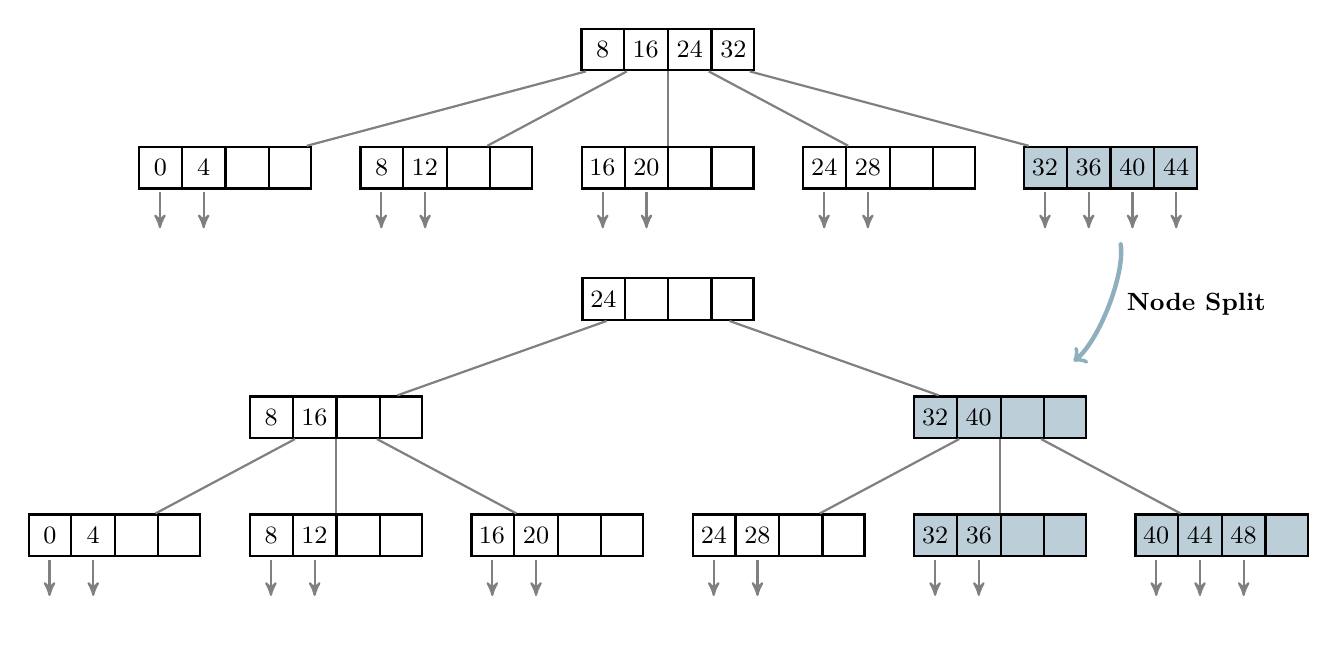
\begin{tikzpicture}
\tikzstyle{trans} = [gray,->,thick,>=stealth',shorten <=1pt,shorten >=1pt]
\tikzstyle{node_style} = [rectangle split,rectangle split horizontal,
  rectangle split parts=4,rectangle split empty part width=10.5pt,
  text width=15pt,inner sep=0,thick,draw=black,
  minimum height=15pt,text centered,anchor=center,font=\small]
\tikzstyle{edge_style} = [gray,thick,draw]
\tikzstyle{level 1}=[sibling distance=80pt]

\uncover<1->{
\begin{scope} [local bounding box=scope1,%edge from parent fork down,
  every node/.style=node_style, edge from parent/.style=edge_style]
\node {8 \nodepart{two} 16 \nodepart{three} 24 \nodepart{four} 32}
  child {node (l1_0) {0 \nodepart{two} 4}}
  child {node (l1_1) {8 \nodepart{two} 12}}
   child {node (l1_2) {16 \nodepart{two} 20}}
   child {node (l1_3) {24 \nodepart{two} 28}}
   child {node[fill=paperblue!30] (l1_4) {32 \nodepart{two} 36 \nodepart{three} 40 \nodepart{four} 44}};
\end{scope}

\foreach \i in {0,...,4} {
\node[below=15pt of l1_\i.one south] (c\i) {};
\draw[trans] (l1_\i.one south) -- (c\i);
\node[below=15pt of l1_\i.two south] (c\i_2) {};
\draw[trans] (l1_\i.two south) -- (c\i_2);
}
% Last two arrows
\node[below=15pt of l1_4.three south] (c4_3) {};
\draw[trans] (l1_4.three south) -- (c4_3);
\node[below=15pt of l1_4.four south] (c4_4) {};
\draw[trans] (l1_4.four south) -- (c4_4);
}

\uncover<3->{
\begin{scope}[shift={($(scope1.south)+(0,-40pt)$)},%edge from parent fork down,
  every node/.style=node_style, edge from parent/.style=edge_style]
\tikzstyle{level 1}=[sibling distance=240pt]
\tikzstyle{level 2}=[sibling distance=80pt]
\node {24}
  child {node {8 \nodepart{two} 16}
    child {node (l2_0) {0 \nodepart{two} 4}}
    child {node (l2_1) {8 \nodepart{two} 12}}
    child {node (l2_2) {16 \nodepart{two} 20}}
  }
  child {node[fill=paperblue!30] (l2_split) {32 \nodepart{two} 40}
    child {node (l2_3) {24 \nodepart{two} 28}}
    child {node[fill=paperblue!30] (l2_4) {32 \nodepart{two} 36}}
    child {node[fill=paperblue!30] (l2_5) {40 \nodepart{two} 44 \nodepart{three} 48}}
  };
\end{scope}

\foreach \i in {0,...,5} {
\node[below=15pt of l2_\i.one south] (c\i) {};
\draw[trans] (l2_\i.one south) -- (c\i);
\node[below=15pt of l2_\i.two south] (c\i_2) {};
\draw[trans] (l2_\i.two south) -- (c\i_2);
}
% Last arrow
\node[below=15pt of l2_5.three south] (c5_3) {};
\draw[trans] (l2_5.three south) -- (c5_3);
}

\uncover<2->{
\draw[overlay,remember picture,ultra thick,line cap=round,->,
  draw=paperblue!50,shorten <=20pt,shorten >=20pt] (l1_4) to [bend left=30]
  node[right=5pt, font=\small\bfseries] {Node Split} 
  (l2_split);
}
\end{tikzpicture}


\caption{Simplified version of original B-tree structure used for indexing 
chunks. In the case of extendable datasets, whenever a new chunk is added to 
the B-tree, its right-most node, if full, is split and a new half empty node 
is created.}
\label{fig:btree1}
\end{figure*}

Chunking is a technique used in the HDF5 library in various cases:
to optimize I/O to disk~\cite{Howison2010}, to compress data~\cite{Folk2011},
to extend datasets.
To retrieve elements in the datasets that are stored in chunked form, the
chunk containing those elements must be located and accessed.
The HDF5 library's default data structure for indexing chunks is based on
a B-tree data structure, which maps the coordinate offset of the chunk to the
file offset where the chunk's elements are stored.

\subsection{B-Trees}

B-trees are generally used for indexing data blocks
and are one of the main components of file systems~\cite{Comer1979}~\cite{Folk1992}. 
Insertion of a new entry and lookup is realized in $O(\log_b{n})$, where $n$ is the
number of nodes and $b$ the order of the tree.
In the case of HDF5 datasets and in the original B-tree structure, referred to
as \textit{B-Tree version 1} (BT1), the record for locating a chunk stores the
following information:
\begin{itemize}
\item The coordinates of the chunk in the dataset's dataspace. This is used
as the key for locating chunks in the B-tree.
\item The size of the chunk, in bytes.
\item The address of the chunk in the file.
\item Additional metadata.
\end{itemize}

%One of the first issues is the redundancy of chunk size,
%inserted in every record, as the chunks are fixed size.
As shown in figure~\ref{fig:btree1}, each leaf points to the address of a
chunk. When a dataset is extended, a new entry is added, which may
generate a node split if the node where the record needs to be inserted is full. 
It is worth noting that most chunked datasets are either fixed dimension or
extend in only one dimension---very few users take advantage of the ability to 
extend multiple dimensions of a dataset.

Because HDF5 datasets only allow their dimensions to be increased or 
decreased at their upper bound, a B-tree used to index chunks for a 1-D 
dataset will only ever insert or remove records from its right-most node.
One of the problems this causes is that inserting/removing only from the right-most
node lets most records half empty, as illustrated in figure~\ref{fig:btree1}.
To fix that issue, one of the main improvements made with a new version of
the B-tree structure used, referred to as \textit{B-tree version 2} (BT2), is to
re-balance the entries so that nodes that were half-empty in version 1 are
now full.
%Additionally, to improve traversal of the tree and easily find the
%chunks, the B-tree is counted so that alongside every link to a subtree, the
%number of subtree elements is stored.
Some additional modifications have also been made to the BT2 to improve performance:
\begin{enumerate}
\item
When appending to a dataset, the library will insert a new record to the
B-tree. To determine that the record to be inserted is not in the tree,
the library traverses the corresponding tree nodes and compares the records 
in each node before the insertion.
To accelerate the search, the maximum and minimum records in the tree are 
determined and stored in memory. The library can then quickly 
determine that the new record to be inserted is not in the tree if it is 
greater than the maximum record or less than the minimum record.
\item
The default BT2 node size is $512$, which leads to a greater tree depth
than version 1 for the append test scenario. This contributes to a lower
performance because the traversal time is increased. The node size for the
tree is therefore modified to $2048$, which will flatten the tree with a tree 
depth that is the same as the BT1.
\end{enumerate}

\subsection{Extensible Arrays}
While the version 2 B-tree previously mentioned provides a better
balancing of the records in the tree, using it in the 1-D case (or for
datasets with only one unlimited dimension) still only ever inserts or removes
records from the right-most node.
This negates most of the advantage of using a complicated data structure like a
B-tree to index the chunks.
Additionally, for applications, which wish to rapidly append records to the 
dataset, having to traverse and/or update multiple B-tree nodes for each 
record insertion imposes an additional performance penalty. This is 
especially a drawback when splitting one or more B-tree nodes is required to 
accommodate new record for a chunk.

\begin{figure*}
\centering
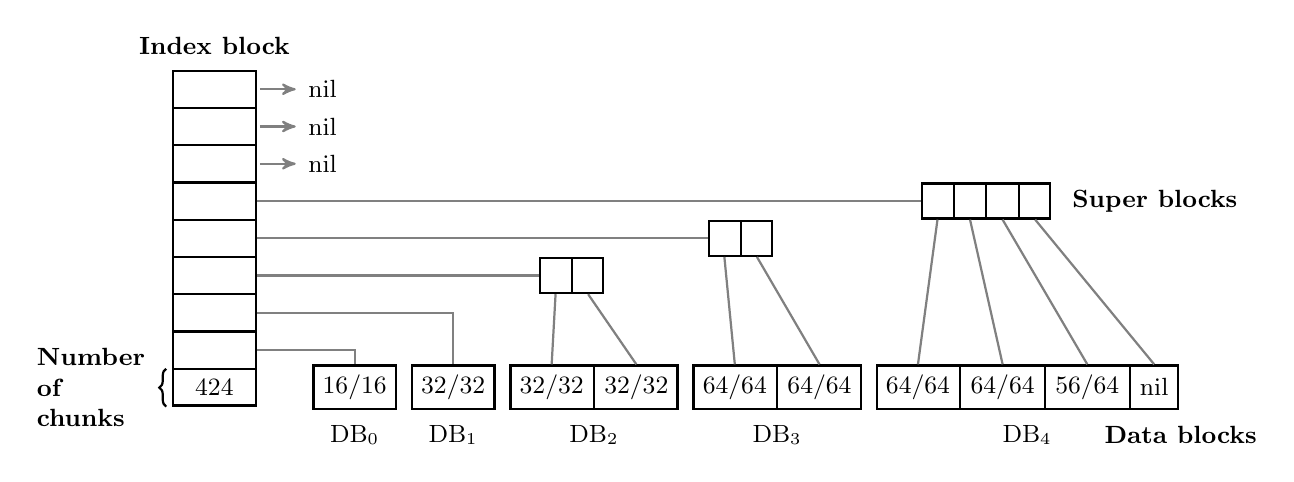
\begin{tikzpicture}
\tikzstyle{sblock} = [rectangle split,rectangle split horizontal,
  rectangle split empty part height=6pt,thick,draw=black,
  minimum width=30pt,text centered,font=\small,
  anchor=center]
\tikzstyle{iblock} = [rectangle split,rectangle split parts=9,
  rectangle split empty part height=6pt,thick,draw=black,
  minimum width=30pt,text centered,font=\small,
  anchor=center]
\tikzstyle{link} = [gray,thick,draw]
\tikzstyle{trans} = [gray,->,thick,>=stealth',shorten <=1pt,shorten >=1pt]
\tikzstyle{annotation} = [font=\small]

\node[iblock] (index) {~\nodepart{two}~\nodepart{three}~\nodepart{four}~\nodepart{five}~\nodepart{six}~\nodepart{seven}~\nodepart{eight}~\nodepart{nine}424};
\node[sblock,rectangle split parts=1,right=20pt of index.nine east] (sblock0) {16/16};
\node[sblock,rectangle split parts=1,right=5pt of sblock0] (sblock1) {32/32};
\node[sblock,rectangle split parts=2,right=5pt of sblock1] (sblock2) {32/32 \nodepart{two} 32/32};
\node[sblock,rectangle split parts=2,right=5pt of sblock2] (sblock3) {64/64 \nodepart{two} 64/64};
\node[sblock,rectangle split parts=4,right=5pt of sblock3] (sblock4) {64/64 \nodepart{two} 64/64 \nodepart{three} 56/64 \nodepart{four} nil};
\node[sblock,rectangle split parts=2,right=102pt of index.six east] (sblock2b) {};
\node[sblock,rectangle split parts=2,right=163pt of index.five east] (sblock3b) {};
\node[sblock,rectangle split parts=4,right=240pt of index.four east] (sblock4b) {};

\draw[link] (index.eight east) -| (sblock0);
\draw[link] (index.seven east) -| (sblock1);
\draw[link] (index.six east) -- (sblock2b);
\draw[link] (index.five east) -- (sblock3b);
\draw[link] (index.four east) -- (sblock4b);

\draw[link] (sblock2b.one south) -- (sblock2.one north);
\draw[link] (sblock2b.two south) -- (sblock2.two north);

\draw[link] (sblock3b.one south) -- (sblock3.one north);
\draw[link] (sblock3b.two south) -- (sblock3.two north);

\draw[link] (sblock4b.one south) -- (sblock4.one north);
\draw[link] (sblock4b.two south) -- (sblock4.two north);
\draw[link] (sblock4b.three south) -- (sblock4.three north);
\draw[link] (sblock4b.four south) -- (sblock4.four north);

\node[annotation,right=15pt of index.one east] (nil0) {nil};
\draw[trans] (index.one east) -- (nil0);
\node[annotation,right=15pt of index.two east] (nil1) {nil};
\draw[trans] (index.two east) -- (nil1);
\node[annotation,right=15pt of index.three east] (nil2) {nil};
\draw[trans] (index.three east) -- (nil2);

\uncover<3->{
\draw[decorate,decoration={brace,mirror,raise=2pt}, thick] (index.eight split west) to node [annotation,text width=40pt,left=5pt,font=\small\bfseries] {Number of chunks} (index.south west);
}
\node[annotation,below=2pt of sblock0] {DB$_0$};
\node[annotation,below=2pt of sblock1] {DB$_1$};
\node[annotation,below=2pt of sblock2] {DB$_2$};
\node[annotation,below=2pt of sblock3] {DB$_3$};
\node[annotation,below=2pt of sblock4] (sblock4_annotation) {DB$_4$};
\uncover<2->{
\node[annotation,above=2pt of index,font=\small\bfseries] {Index block};
}
\uncover<5->{
\node[annotation,right=12pt of sblock4_annotation,font=\small\bfseries] {Data blocks};
}
\uncover<4->{
\node[annotation,right=4pt of sblock4b,font=\small\bfseries] {Super blocks};
}

% To help center
%\node[above=100pt of sblock2.one split] (help2) {};
%\draw (help2) -- (sblock2.one split);
%\node[above=100pt of sblock3.one split] (help3) {};
%\draw (help3) -- (sblock3.one split);
%\node[above=100pt of sblock4.two split] (help4) {};
%\draw (help4) -- (sblock4.two split);
\end{tikzpicture}


\caption{Simplified version of extensible array structure used for indexing chunks.}
\label{fig:ea}
\end{figure*}

For this particular case, indexing chunks requires a more appropriate data
structure, referred to as \textit{extensible array} (EA), and shown in
figure~\ref{fig:ea}. This structure can be seen as a dynamic array structure,
which can contain new elements, as needed---insertion, removal and lookup of
elements are realized in constant time.
Brodnik et al's paper~\cite{Brodnik1999} shows how to implement a similar
structure with $O(1)$ append, shrink and lookup
operations, along with optimal metadata overhead for indexing the array elements.
In our case and for indexing chunks in HDF5 datasets, the array elements in the
data blocks are pointers to the chunks on disk.
To conceptually group the data blocks that the index block points to,
the extensible array defines \textit{super blocks}.
Super blocks are not actually constructs in the data structure, but
as mentioned in~\cite{Brodnik1999}, help to show the pattern of
changes to the data blocks: first the size of the data block doubles, then the 
number of data blocks of that size doubles, then the size doubles again, then the 
number of data blocks of that size doubles, etc.

A couple of things should be noted about this data structure (described in
figure~\ref{fig:ea}):
\begin{enumerate}
\item The super blocks for the first two data blocks are omitted and the pointers
in the index block point directly to the data blocks.
\item Constant time (i.e., $O(1)$) lookup, append and shrink are still in effect.
The number of I/O accesses to find any chunk address is always $2$ or $3$:
index block $\rightarrow$ super block $\rightarrow$ data block. In
actual operation, the index block will certainly be \textit{hot} enough to stay
in the HDF5 metadata cache, along with many/most of the super blocks,
making the average number of I/O accesses to retrieve a chunk address between
$1$ and $2$, in all likelihood.
\item Super blocks/data blocks, which are not yet needed, are not allocated and
have a \textit{nil} pointer in the index block/super block (respectively) that
refers to them.
\item The height of the index block is constant and its height can be computed
at creation so that resizing it is unnecessary. This can be done by computing
the maximum number of chunks possible for the file's address range
(typically 64-bits) and deriving the maximum number of data/index blocks needed
to index that many blocks. For example, if there are $16$ chunks in the initial
data block, a chunk size of $2048$ (with a single unlimited dimension), and a
4-byte (integer) data element size, the maximum height of the index block needed to
store $1.84\times 10^{19}$ bytes of elements (which is the maximum offset
possible in a 64-bit file) is $46$:
\begin{align*}
16\times \sum_{i=0}^{n} 2^{i} = \frac{2^{64}}{2048 \times 4}\\
16\times (2^{n+1}-1) = \frac{2^{64}}{2048 \times 4}\\
2^{n+1} = \frac{2^{64}}{2048 \times 4 \times 16} + 1\\
2^{n+1} = 2^{47} + 1\\
\lceil n \rceil = 46
\end{align*}
\end{enumerate}

%Look at H5D_chunk_hashval / H5D_set_extent
\subsection{Hash Table}
In the case where chunks are present in cache (i.e., in memory),
chunks are retrieved from the cache hash table. When a dataset's dimensions are
extended and the dataset's rank is greater than one, the HDF5 library scans
and updates each entry in the chunk cache, due to the modified dataspace.
In the original implementation, each entry is hashed based on the chunk index,
which varies according to the dataset dimension sizes. When the dimension sizes
are modified, the library re-calculates each entry's chunk index and updates
the cache accordingly. This is an expensive operation since the update time
increases as the number of entries is increased in the cache.

To improve performance of chunk retrieval from the cache, two
modifications are made to the chunk layer:
\begin{enumerate}
\item The fastest changing dimension in the chunk index calculation is saved after
initial computation so that it can be later used when updating the chunk cache.
\item A different formula to hash chunk entries into the cache is used so that
it no longer depends on the chunk index. The new formula is based on the
$\log_2$ function, which reduces the number of chunk cache
updates due to consecutive dataset extension operations. As shown
in figure~\ref{fig:scaled}, using scaled coordinates (i.e., relative to the
dimension sizes), the $\log_2$ function is used to compute
a binary representation of the coordinates. The number of bits that are necessary
to encode the coordinates only increases when the new dimension's size crosses
a power of 2 boundary.
\end{enumerate}

\begin{figure*}
\centering
\tikzstyle{trans} = [>=stealth, thick, text centered, font=\small]
\tikzstyle{computBox} = [draw=black, thick, inner sep=4pt, inner ysep=4pt,
  rectangle, rounded corners]

\newcommand{\drawcuboid}[5]{% width, height, depth, scale, color
\begin{scope}[scale=#4]
\coordinate (O) at (0,0,0);
\coordinate (A) at (0,#2,0);
\coordinate (B) at (0,#2,#3);
\coordinate (C) at (0,0,#3);
\coordinate (D) at (#1,0,0);
\coordinate (E) at (#1,#2,0);
\coordinate (F) at (#1,#2,#3);
\coordinate (G) at (#1,0,#3);

\draw[fill=#5] (O) -- (C) -- (G) -- (D) -- cycle;% Bottom Face
\draw[fill=#5] (O) -- (A) -- (E) -- (D) -- cycle;% Back Face
\draw[fill=#5] (O) -- (A) -- (B) -- (C) -- cycle;% Left Face
\draw[fill=#5] (D) -- (E) -- (F) -- (G) -- cycle;% Right Face
\draw[fill=#5] (C) -- (B) -- (F) -- (G) -- cycle;% Front Face
\draw[fill=#5] (A) -- (B) -- (F) -- (E) -- cycle;% Top Face

\draw[dashed] (O) -- (D);
\draw[dashed] (O) -- (C);
\draw[dashed] (O) -- (A);

\coordinate[left=6pt of A] (A1);
\coordinate[left=6pt of B] (B1);
\coordinate[left=6pt of C] (C1);
\coordinate[below=4pt of C] (C2);
\coordinate[below=4pt of G] (G1);
\draw[<->,trans] (C2) -- node [below] {#1} (G1);
\draw[<->,trans] (C1) -- node [left] {#2} (B1);
\draw[<->,trans] (A1) -- node [above left] {#3} (B1);

\end{scope}
}

%\DeclarePairedDelimiter\ceil{\lceil}{\rceil}

\begin{tikzpicture}

\node (cubes) {
\begin{minipage}{0.32\textwidth}
\begin{tikzpicture}
% Origin axes
\draw[->,draw=paperblue,thick] (0,0,0) -- (3.2,0,0);
\draw[->,draw=paperblue,thick] (0,0,0) -- (0,3.8,0);
\draw[->,draw=paperblue,thick] (0,0,0) -- (0,0,4);
\node[font=\itshape] at (3.4,0,0) {x};
\node[font=\itshape] at (0,4,0) {y};
\node[font=\itshape] at (0,0,4.2) {z};

% Cubes
\drawcuboid{60}{75}{75}{0.04}{white}
\drawcuboid{10}{25}{25}{0.04}{paperblue!20}
\end{tikzpicture}
\end{minipage}
};

% Hash value computation
\node [computBox, font=\footnotesize, text width=100pt, right=50pt of cubes] (scaled) {
  \begin{minipage}{\textwidth}
  {
\textbf{Scaled coordinates:}\\
\begin{math}
   X/x = 60/10 = 6\\
   Y/y = 75/25 = 3\\
   Z/z = 75/25 = 3
\end{math}

\smallskip
\textbf{Number of bits to represent\\ coordinates:}\\
\begin{math}
   \lceil \log_2(X/x) \rceil = 3\\
   \lceil \log_2(Y/y) \rceil = 2\\
   \lceil \log_2(Z/z) \rceil = 2
\end{math}
  }
  \end{minipage}
};

\node [right=of scaled,rectangle split,rectangle split horizontal,
  rectangle split parts=2,draw, minimum height=15pt,text centered,anchor=center,font=\small] (zhash) {0 \nodepart{two} 0};
\node [right=14pt of zhash,rectangle split,rectangle split horizontal,
  rectangle split parts=2,draw, minimum height=15pt,text centered,anchor=center,font=\small] (yhash) {0 \nodepart{two} 0};
\node [right=20pt of yhash,rectangle split,rectangle split horizontal,
  rectangle split parts=3,draw, minimum height=15pt,text centered,anchor=center,font=\small] (xhash) {0 \nodepart{two} 0 \nodepart{three} 0};
\node [below=2pt of xhash] {$x$};
\node [below=2pt of yhash] {$y$};
\node [below=2pt of zhash] {$z$};

\draw[very thick, ->] (cubes) -- node[above, text width=4cm, align=center, font=\bfseries]
    {Hash-value} ($ (scaled.west) - (0.5,0) $);

\end{tikzpicture}



\caption{Example of hash-value computation that is used to retrieve chunks using
 scaled coordinates in a 3-dimensional dataset.}
\label{fig:scaled}
\end{figure*}

\subsection{Summary}

With these data structures in place, when the chunked dataset is on disk and
has only one unlimited maximum dimension, the extensible array indexing method is used,
allowing chunk access in $O(1)$ time. When it has more than one unlimited
maximum dimension sizes, the B-tree version 2 indexing method is used, allowing
chunk access in $O(\log_b{n})$, with $b$ the order of the tree and $n$ the
number of nodes. When it is in cache, the chunk is accessed through the cache
hash table and the computed hash value.

\section{Evaluation}
\label{sec:evaluation}

To evaluate the performance of these new methods, we first consider the extension
of datasets so that 1-byte chunks are appended, up to $2,500,000$ bytes.
Note that the default storage for chunked datasets is still the default
B-tree indexing (BT1). In order to retain as much forward compatibility as
possible, all the improvements made are only used when the
\texttt{H5F\_LIBVER\_LATEST} value is used as the \textit{high bound} to the
call to \texttt{H5Pset\_libver\_bounds}, which can be set by an application
when the file is opened.

\subsection{Test Scenarios}

We consider multiple scenarios, which are defined in settings 1, 2 and 3.

\paragraph{Setting 1}
creates a 1-dimensional chunked dataset with the following dataspace:

{\lstsetc
\begin{lstlisting}
curr[0] = 0;
max[0] = H5S_UNLIMITED;
sid = H5Screate_simple(1, curr, max);
\end{lstlisting}
}

This compares the BT1 and EA indexing methods, when appending to the dataset
created with the old and new library format respectively.

\paragraph{Setting 2} creates a 2-dimensional chunked dataset with the following
dataspace, which has one unlimited dimension:

{\lstsetc
\begin{lstlisting}
curr[0] = 0;
curr[1] = 1;
max[0] = H5S_UNLIMITED;
max[1] = 1;
sid = H5Screate_simple(2, curr, max);
\end{lstlisting}
}

This compares the BT1 and EA indexing methods when appending to the dataset
created with the old and the new library format respectively.
Append operations are done along the X or Y directions.

\paragraph{Setting 3} creates 2-dimensional chunked datasets with the following
dataspace, which has two unlimited dimensions:

{\lstsetc
\begin{lstlisting}
curr[0] = 0;
curr[1] = 1;
max[0] = H5S_UNLIMITED;
max[1] = H5S_UNLIMITED;
sid = H5Screate_simple(2, curr, max);
\end{lstlisting}
}

This compares the BT1 and BT2 indexing methods when appending to the
datasets created with the old and new library format respectively.
Append operations are done along the X and/or Y directions.

\subsection{Preliminary Results}

First, measures are realized on the library before optimization.
The quantify tool is used to collect the time in seconds spent in the library
code from the test runs. The result listed in table~\ref{tab:result1} indicates
that the EA indexing method performs better than BT1, while the BT2 indexing
method performs worse than BT1. Note also that the library takes a fair amount
of time for all three indexing methods.

\begin{table}
\centering
\caption{Result for all three test settings before optimization.}
\label{tab:result1}
\begin{tabular}{lrr} \toprule
Indexing Method &
Time (\si{\second}) \\
\midrule
\textit{Along the X-direction} \\
EA & $149.82$\tikzmark{t1x1} \\
BT1 & $156.15$\tikzmark{t1x2} \\
BT2 & $166.56$\tikzmark{t1x3} \\
\midrule
\textit{Along the Y-direction} \\
EA & $150.08$\tikzmark{t1y1} \\
BT1 & $163.82$\tikzmark{t1y2} \\
BT2 & $167.91$\tikzmark{t1y3} \\
\midrule
\textit{Along the XY-direction} \\
EA & $-$ \\
BT1 & $104.08$\tikzmark{t1xy1} \\
BT2 & $114.39$\tikzmark{t1xy2} \\
\bottomrule
\end{tabular}
\tablearrowright{t1x2}{t1x1}{$\simeq -4\%$}{}
\tablearrowleft{t1x2}{t1x3}{$\simeq +7\%$}{}
\tablearrowright{t1y2}{t1y1}{$\simeq -8\%$}{}
\tablearrowleft{t1y2}{t1y3}{$\simeq +2\%$}{}
\tablearrowleft{t1xy1}{t1xy2}{$\simeq +10\%$}{}
\end{table}

\subsection{Results}
Measures are realized after optimization.
The new results shown in table~\ref{tab:result2} indicate that after optimization
BT2 performs better than BT1. General chunk index fixes have made a significant
improvement for all three indexing methods---almost $80\%$.

\begin{table}
\centering
\caption{Result for all three test settings after optimization.}
\label{tab:result2}
\begin{tabular}{lr} \toprule
Indexing Method &
Time (\si{\second}) \\
\midrule
\textit{Along the X-direction} \\
EA & $32.10$\tikzmark{x1}\\
BT1 & $36.63$\tikzmark{x2} \\
BT2 & $35.39$\tikzmark{x3} \\
\midrule
\textit{Along the Y-direction} \\
EA & $32.2$\tikzmark{y1} \\
BT1 & $39.01$\tikzmark{y2} \\
BT2 & $34.90$\tikzmark{y3} \\
\midrule
\textit{Along the XY-direction} \\
EA & $-$ \\
BT1 & $36.11$\tikzmark{xy1} \\
BT2 & $35.29$\tikzmark{xy2} \\
\bottomrule
\end{tabular}
\tablearrowright{x2}{x1}{$\simeq -12.4\%$}{}
\tablearrowleft{x2}{x3}{$\simeq -3.4\%$}{fill=paperblue!30}
\tablearrowright{y2}{y1}{$\simeq -17.5\%$}{}
\tablearrowleft{y2}{y3}{$\simeq -10.5\%$}{fill=paperblue!30}
\tablearrowleft{xy1}{xy2}{$\simeq -2.3\%$}{fill=paperblue!30}
\end{table}

As one can see in figure~\ref{fig:chunk_perf}, for significant numbers of chunks,
the BT2 and EA indexing methods perform better than BT1. EA shows good scalability
and a much better performance than BT1/BT2 as the number of chunks increases.
BT2 generally shows better performance than BT1 (it is also worth noting than
even if this is not shown in this result, the amount of space taken by BT2
is reduced). Overall these results confirm the optimization made within the
library and were what we expected given the complexity of the methods used.

\begin{figure*}
\centering
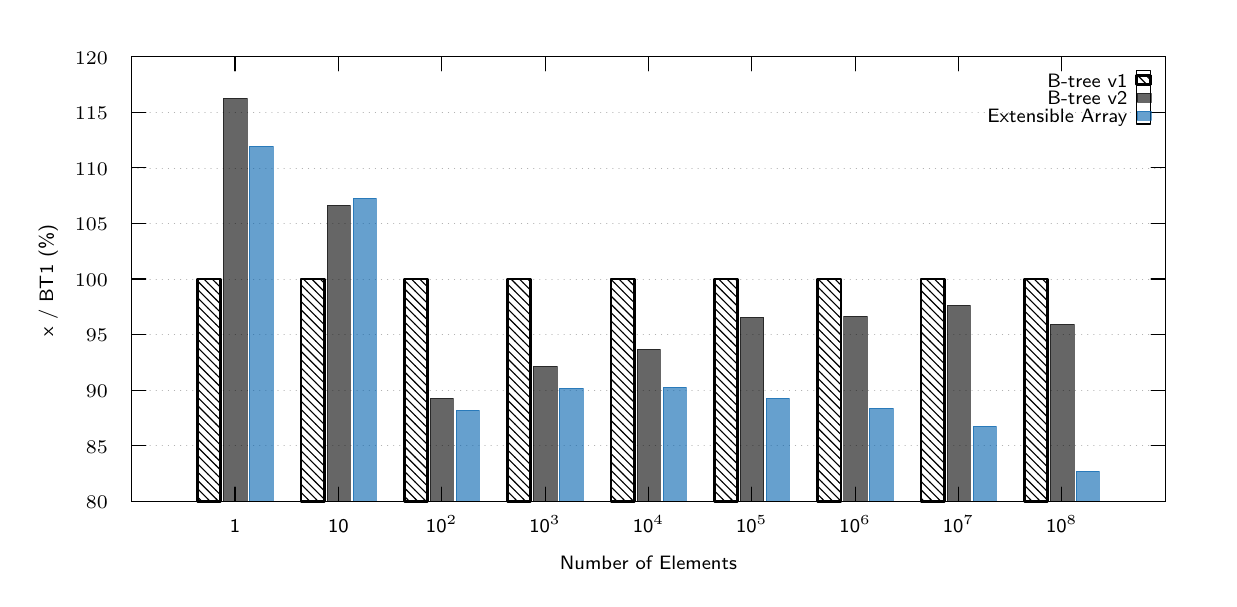
\begin{tikzpicture}[gnuplot]
%% generated with GNUPLOT 5.0p0 (Lua 5.3; terminal rev. 99, script rev. 100)
%% Tue 09 Jun 2015 04:43:46 PM CDT
\tikzset{every node/.append style={font={\sffamily\scriptsize}}}
\path (0.000,0.000) rectangle (15.000,7.000);
\gpcolor{color=gp lt color axes}
\gpsetlinetype{gp lt axes}
\gpsetdashtype{gp dt axes}
\gpsetlinewidth{0.50}
\draw[gp path] (1.320,0.985)--(14.447,0.985);
\gpcolor{color=gp lt color border}
\gpsetlinetype{gp lt border}
\gpsetdashtype{gp dt solid}
\gpsetlinewidth{1.00}
\draw[gp path] (1.320,0.985)--(1.500,0.985);
\draw[gp path] (14.447,0.985)--(14.267,0.985);
\node[gp node right,font={\sffamily\scriptsize}] at (1.136,0.985) {$80$};
\gpcolor{color=gp lt color axes}
\gpsetlinetype{gp lt axes}
\gpsetdashtype{gp dt axes}
\gpsetlinewidth{0.50}
\draw[gp path] (1.320,1.691)--(14.447,1.691);
\gpcolor{color=gp lt color border}
\gpsetlinetype{gp lt border}
\gpsetdashtype{gp dt solid}
\gpsetlinewidth{1.00}
\draw[gp path] (1.320,1.691)--(1.500,1.691);
\draw[gp path] (14.447,1.691)--(14.267,1.691);
\node[gp node right,font={\sffamily\scriptsize}] at (1.136,1.691) {$85$};
\gpcolor{color=gp lt color axes}
\gpsetlinetype{gp lt axes}
\gpsetdashtype{gp dt axes}
\gpsetlinewidth{0.50}
\draw[gp path] (1.320,2.397)--(14.447,2.397);
\gpcolor{color=gp lt color border}
\gpsetlinetype{gp lt border}
\gpsetdashtype{gp dt solid}
\gpsetlinewidth{1.00}
\draw[gp path] (1.320,2.397)--(1.500,2.397);
\draw[gp path] (14.447,2.397)--(14.267,2.397);
\node[gp node right,font={\sffamily\scriptsize}] at (1.136,2.397) {$90$};
\gpcolor{color=gp lt color axes}
\gpsetlinetype{gp lt axes}
\gpsetdashtype{gp dt axes}
\gpsetlinewidth{0.50}
\draw[gp path] (1.320,3.102)--(14.447,3.102);
\gpcolor{color=gp lt color border}
\gpsetlinetype{gp lt border}
\gpsetdashtype{gp dt solid}
\gpsetlinewidth{1.00}
\draw[gp path] (1.320,3.102)--(1.500,3.102);
\draw[gp path] (14.447,3.102)--(14.267,3.102);
\node[gp node right,font={\sffamily\scriptsize}] at (1.136,3.102) {$95$};
\gpcolor{color=gp lt color axes}
\gpsetlinetype{gp lt axes}
\gpsetdashtype{gp dt axes}
\gpsetlinewidth{0.50}
\draw[gp path] (1.320,3.808)--(14.447,3.808);
\gpcolor{color=gp lt color border}
\gpsetlinetype{gp lt border}
\gpsetdashtype{gp dt solid}
\gpsetlinewidth{1.00}
\draw[gp path] (1.320,3.808)--(1.500,3.808);
\draw[gp path] (14.447,3.808)--(14.267,3.808);
\node[gp node right,font={\sffamily\scriptsize}] at (1.136,3.808) {$100$};
\gpcolor{color=gp lt color axes}
\gpsetlinetype{gp lt axes}
\gpsetdashtype{gp dt axes}
\gpsetlinewidth{0.50}
\draw[gp path] (1.320,4.514)--(14.447,4.514);
\gpcolor{color=gp lt color border}
\gpsetlinetype{gp lt border}
\gpsetdashtype{gp dt solid}
\gpsetlinewidth{1.00}
\draw[gp path] (1.320,4.514)--(1.500,4.514);
\draw[gp path] (14.447,4.514)--(14.267,4.514);
\node[gp node right,font={\sffamily\scriptsize}] at (1.136,4.514) {$105$};
\gpcolor{color=gp lt color axes}
\gpsetlinetype{gp lt axes}
\gpsetdashtype{gp dt axes}
\gpsetlinewidth{0.50}
\draw[gp path] (1.320,5.220)--(14.447,5.220);
\gpcolor{color=gp lt color border}
\gpsetlinetype{gp lt border}
\gpsetdashtype{gp dt solid}
\gpsetlinewidth{1.00}
\draw[gp path] (1.320,5.220)--(1.500,5.220);
\draw[gp path] (14.447,5.220)--(14.267,5.220);
\node[gp node right,font={\sffamily\scriptsize}] at (1.136,5.220) {$110$};
\gpcolor{color=gp lt color axes}
\gpsetlinetype{gp lt axes}
\gpsetdashtype{gp dt axes}
\gpsetlinewidth{0.50}
\draw[gp path] (1.320,5.925)--(14.083,5.925);
\draw[gp path] (14.263,5.925)--(14.447,5.925);
\gpcolor{color=gp lt color border}
\gpsetlinetype{gp lt border}
\gpsetdashtype{gp dt solid}
\gpsetlinewidth{1.00}
\draw[gp path] (1.320,5.925)--(1.500,5.925);
\draw[gp path] (14.447,5.925)--(14.267,5.925);
\node[gp node right,font={\sffamily\scriptsize}] at (1.136,5.925) {$115$};
\gpcolor{color=gp lt color axes}
\gpsetlinetype{gp lt axes}
\gpsetdashtype{gp dt axes}
\gpsetlinewidth{0.50}
\draw[gp path] (1.320,6.631)--(14.447,6.631);
\gpcolor{color=gp lt color border}
\gpsetlinetype{gp lt border}
\gpsetdashtype{gp dt solid}
\gpsetlinewidth{1.00}
\draw[gp path] (1.320,6.631)--(1.500,6.631);
\draw[gp path] (14.447,6.631)--(14.267,6.631);
\node[gp node right,font={\sffamily\scriptsize}] at (1.136,6.631) {$120$};
\draw[gp path] (2.633,0.985)--(2.633,1.165);
\draw[gp path] (2.633,6.631)--(2.633,6.451);
\node[gp node center,font={\sffamily\scriptsize}] at (2.633,0.677) {1};
\draw[gp path] (3.945,0.985)--(3.945,1.165);
\draw[gp path] (3.945,6.631)--(3.945,6.451);
\node[gp node center,font={\sffamily\scriptsize}] at (3.945,0.677) {10};
\draw[gp path] (5.258,0.985)--(5.258,1.165);
\draw[gp path] (5.258,6.631)--(5.258,6.451);
\node[gp node center,font={\sffamily\scriptsize}] at (5.258,0.677) {10$^2$};
\draw[gp path] (6.571,0.985)--(6.571,1.165);
\draw[gp path] (6.571,6.631)--(6.571,6.451);
\node[gp node center,font={\sffamily\scriptsize}] at (6.571,0.677) {10$^3$};
\draw[gp path] (7.884,0.985)--(7.884,1.165);
\draw[gp path] (7.884,6.631)--(7.884,6.451);
\node[gp node center,font={\sffamily\scriptsize}] at (7.884,0.677) {10$^4$};
\draw[gp path] (9.196,0.985)--(9.196,1.165);
\draw[gp path] (9.196,6.631)--(9.196,6.451);
\node[gp node center,font={\sffamily\scriptsize}] at (9.196,0.677) {10$^5$};
\draw[gp path] (10.509,0.985)--(10.509,1.165);
\draw[gp path] (10.509,6.631)--(10.509,6.451);
\node[gp node center,font={\sffamily\scriptsize}] at (10.509,0.677) {10$^6$};
\draw[gp path] (11.822,0.985)--(11.822,1.165);
\draw[gp path] (11.822,6.631)--(11.822,6.451);
\node[gp node center,font={\sffamily\scriptsize}] at (11.822,0.677) {10$^7$};
\draw[gp path] (13.134,0.985)--(13.134,1.165);
\draw[gp path] (13.134,6.631)--(13.134,6.451);
\node[gp node center,font={\sffamily\scriptsize}] at (13.134,0.677) {10$^8$};
\draw[gp path] (1.320,6.631)--(1.320,0.985)--(14.447,0.985)--(14.447,6.631)--cycle;
\node[gp node center,rotate=-270,font={\sffamily\scriptsize}] at (0.246,3.808) {x / BT1 (\%)};
\node[gp node center,font={\sffamily\scriptsize}] at (7.883,0.215) {Number of Elements};
\draw[gp path] (14.083,5.776)--(14.083,6.451)--(14.263,6.451)--(14.263,5.776)--cycle;
\node[gp node right,font={\sffamily\fontsize{7.0pt}{8.4pt}\selectfont}] at (14.083,6.338) {B-tree v1};
\def\gpfillpath{(14.083,6.282)--(14.263,6.282)--(14.263,6.394)--(14.083,6.394)--cycle}
\gpfill{color=gpbgfillcolor} \gpfillpath;
\gpfill{rgb color={0.000,0.000,0.000},gp pattern 2,pattern color=.} \gpfillpath;
\gpcolor{rgb color={0.000,0.000,0.000}}
\gpsetlinewidth{2.50}
\draw[gp path] (14.083,6.282)--(14.263,6.282)--(14.263,6.394)--(14.083,6.394)--cycle;
\def\gpfillpath{(2.157,0.985)--(2.453,0.985)--(2.453,3.809)--(2.157,3.809)--cycle}
\gpfill{color=gpbgfillcolor} \gpfillpath;
\gpfill{rgb color={0.000,0.000,0.000},gp pattern 2,pattern color=.} \gpfillpath;
\draw[gp path] (2.157,0.985)--(2.157,3.808)--(2.452,3.808)--(2.452,0.985)--cycle;
\def\gpfillpath{(3.470,0.985)--(3.766,0.985)--(3.766,3.809)--(3.470,3.809)--cycle}
\gpfill{color=gpbgfillcolor} \gpfillpath;
\gpfill{rgb color={0.000,0.000,0.000},gp pattern 2,pattern color=.} \gpfillpath;
\draw[gp path] (3.470,0.985)--(3.470,3.808)--(3.765,3.808)--(3.765,0.985)--cycle;
\def\gpfillpath{(4.782,0.985)--(5.079,0.985)--(5.079,3.809)--(4.782,3.809)--cycle}
\gpfill{color=gpbgfillcolor} \gpfillpath;
\gpfill{rgb color={0.000,0.000,0.000},gp pattern 2,pattern color=.} \gpfillpath;
\draw[gp path] (4.782,0.985)--(4.782,3.808)--(5.078,3.808)--(5.078,0.985)--cycle;
\def\gpfillpath{(6.095,0.985)--(6.391,0.985)--(6.391,3.809)--(6.095,3.809)--cycle}
\gpfill{color=gpbgfillcolor} \gpfillpath;
\gpfill{rgb color={0.000,0.000,0.000},gp pattern 2,pattern color=.} \gpfillpath;
\draw[gp path] (6.095,0.985)--(6.095,3.808)--(6.390,3.808)--(6.390,0.985)--cycle;
\def\gpfillpath{(7.408,0.985)--(7.704,0.985)--(7.704,3.809)--(7.408,3.809)--cycle}
\gpfill{color=gpbgfillcolor} \gpfillpath;
\gpfill{rgb color={0.000,0.000,0.000},gp pattern 2,pattern color=.} \gpfillpath;
\draw[gp path] (7.408,0.985)--(7.408,3.808)--(7.703,3.808)--(7.703,0.985)--cycle;
\def\gpfillpath{(8.720,0.985)--(9.017,0.985)--(9.017,3.809)--(8.720,3.809)--cycle}
\gpfill{color=gpbgfillcolor} \gpfillpath;
\gpfill{rgb color={0.000,0.000,0.000},gp pattern 2,pattern color=.} \gpfillpath;
\draw[gp path] (8.720,0.985)--(8.720,3.808)--(9.016,3.808)--(9.016,0.985)--cycle;
\def\gpfillpath{(10.033,0.985)--(10.329,0.985)--(10.329,3.809)--(10.033,3.809)--cycle}
\gpfill{color=gpbgfillcolor} \gpfillpath;
\gpfill{rgb color={0.000,0.000,0.000},gp pattern 2,pattern color=.} \gpfillpath;
\draw[gp path] (10.033,0.985)--(10.033,3.808)--(10.328,3.808)--(10.328,0.985)--cycle;
\def\gpfillpath{(11.346,0.985)--(11.642,0.985)--(11.642,3.809)--(11.346,3.809)--cycle}
\gpfill{color=gpbgfillcolor} \gpfillpath;
\gpfill{rgb color={0.000,0.000,0.000},gp pattern 2,pattern color=.} \gpfillpath;
\draw[gp path] (11.346,0.985)--(11.346,3.808)--(11.641,3.808)--(11.641,0.985)--cycle;
\def\gpfillpath{(12.658,0.985)--(12.955,0.985)--(12.955,3.809)--(12.658,3.809)--cycle}
\gpfill{color=gpbgfillcolor} \gpfillpath;
\gpfill{rgb color={0.000,0.000,0.000},gp pattern 2,pattern color=.} \gpfillpath;
\draw[gp path] (12.658,0.985)--(12.658,3.808)--(12.954,3.808)--(12.954,0.985)--cycle;
\gpcolor{color=gp lt color border}
\node[gp node right,font={\sffamily\fontsize{7.0pt}{8.4pt}\selectfont}] at (14.083,6.113) {B-tree v2};
\gpfill{rgb color={0.000,0.000,0.000},opacity=0.60} (14.083,6.057)--(14.263,6.057)--(14.263,6.169)--(14.083,6.169)--cycle;
\gpfill{rgb color={0.000,0.000,0.000},opacity=0.60} (2.485,0.985)--(2.781,0.985)--(2.781,6.110)--(2.485,6.110)--cycle;
\gpfill{rgb color={0.000,0.000,0.000},opacity=0.60} (3.798,0.985)--(4.094,0.985)--(4.094,4.744)--(3.798,4.744)--cycle;
\gpfill{rgb color={0.000,0.000,0.000},opacity=0.60} (5.110,0.985)--(5.407,0.985)--(5.407,2.297)--(5.110,2.297)--cycle;
\gpfill{rgb color={0.000,0.000,0.000},opacity=0.60} (6.423,0.985)--(6.719,0.985)--(6.719,2.698)--(6.423,2.698)--cycle;
\gpfill{rgb color={0.000,0.000,0.000},opacity=0.60} (7.736,0.985)--(8.032,0.985)--(8.032,2.919)--(7.736,2.919)--cycle;
\gpfill{rgb color={0.000,0.000,0.000},opacity=0.60} (9.049,0.985)--(9.345,0.985)--(9.345,3.331)--(9.049,3.331)--cycle;
\gpfill{rgb color={0.000,0.000,0.000},opacity=0.60} (10.361,0.985)--(10.658,0.985)--(10.658,3.343)--(10.361,3.343)--cycle;
\gpfill{rgb color={0.000,0.000,0.000},opacity=0.60} (11.674,0.985)--(11.970,0.985)--(11.970,3.483)--(11.674,3.483)--cycle;
\gpfill{rgb color={0.000,0.000,0.000},opacity=0.60} (12.987,0.985)--(13.283,0.985)--(13.283,3.240)--(12.987,3.240)--cycle;
\node[gp node right,font={\sffamily\fontsize{7.0pt}{8.4pt}\selectfont}] at (14.083,5.888) {Extensible Array};
\gpfill{rgb color={0.000,0.376,0.678},opacity=0.60} (14.083,5.832)--(14.263,5.832)--(14.263,5.944)--(14.083,5.944)--cycle;
\gpfill{rgb color={0.000,0.376,0.678},opacity=0.60} (2.813,0.985)--(3.110,0.985)--(3.110,5.497)--(2.813,5.497)--cycle;
\gpfill{rgb color={0.000,0.376,0.678},opacity=0.60} (4.126,0.985)--(4.422,0.985)--(4.422,4.837)--(4.126,4.837)--cycle;
\gpfill{rgb color={0.000,0.376,0.678},opacity=0.60} (5.439,0.985)--(5.735,0.985)--(5.735,2.150)--(5.439,2.150)--cycle;
\gpfill{rgb color={0.000,0.376,0.678},opacity=0.60} (6.751,0.985)--(7.048,0.985)--(7.048,2.422)--(6.751,2.422)--cycle;
\gpfill{rgb color={0.000,0.376,0.678},opacity=0.60} (8.064,0.985)--(8.360,0.985)--(8.360,2.437)--(8.064,2.437)--cycle;
\gpfill{rgb color={0.000,0.376,0.678},opacity=0.60} (9.377,0.985)--(9.673,0.985)--(9.673,2.301)--(9.377,2.301)--cycle;
\gpfill{rgb color={0.000,0.376,0.678},opacity=0.60} (10.689,0.985)--(10.986,0.985)--(10.986,2.164)--(10.689,2.164)--cycle;
\gpfill{rgb color={0.000,0.376,0.678},opacity=0.60} (12.002,0.985)--(12.298,0.985)--(12.298,1.942)--(12.002,1.942)--cycle;
\gpfill{rgb color={0.000,0.376,0.678},opacity=0.60} (13.315,0.985)--(13.611,0.985)--(13.611,1.366)--(13.315,1.366)--cycle;
\gpsetlinewidth{1.00}
\draw[gp path] (1.320,6.631)--(1.320,0.985)--(14.447,0.985)--(14.447,6.631)--cycle;
%% coordinates of the plot area
\gpdefrectangularnode{gp plot 1}{\pgfpoint{1.320cm}{0.985cm}}{\pgfpoint{14.447cm}{6.631cm}}
\end{tikzpicture}
%% gnuplot variables

\caption{Performance of BT2 and EA chunk indexing methods compared to BT1.
The extensible array method shows good scaling performance, while the B-Tree
version 2 shows improved results compared to BT1.}
\label{fig:chunk_perf}
\end{figure*}

\section{Related Work}
\label{sec:related_work}

Nimako et al.~\cite{Nimako2012} consider another data structure for indexing
chunks, the $O_{2}$-Tree, which performs query operations (searches) in
$O(\log_{2}{n})$ time, where $n$ is the number of internal nodes. They
mention that the conventional arrays and HDF5 incur the cost
of reorganizing already allocated array elements.
Based on these results and the new optimization made, it would be
interesting to make a new comparison. The $O_{2}$-Tree may perform
better than a B-Tree data structure but the re-sizable array data structure
will still perform better in the 1-unlimited dimension case, as its complexity
is in $O(1)$.

%[Other related work?]
%Sub array I/O from ADIOS etc / chunking from other libraries
%Tell what was done for chunking in the past etc

\section{Conclusion and Future Work}
\label{sec:conclusion}

%\section*{Acknowledgments}
%The work presented in this paper was supported by ???



% trigger a \newpage just before the given reference
% number - used to balance the columns on the last page
% adjust value as needed - may need to be readjusted if
% the document is modified later
%\IEEEtriggeratref{8}
% The "triggered" command can be changed if desired:
%\IEEEtriggercmd{\enlargethispage{-5in}}

% references section

% can use a bibliography generated by BibTeX as a .bbl file
% BibTeX documentation can be easily obtained at:
% http://www.ctan.org/tex-archive/biblio/bibtex/contrib/doc/
% The IEEEtran BibTeX style support page is at:
% http://www.michaelshell.org/tex/ieeetran/bibtex/
\bibliographystyle{IEEEtran}
% argument is your BibTeX string definitions and bibliography database(s)
\bibliography{IEEEabrv,paper}
%
% <OR> manually copy in the resultant .bbl file
% set second argument of \begin to the number of references
% (used to reserve space for the reference number labels box)
%\begin{thebibliography}{1}

%\bibitem{IEEEhowto:kopka}
%H.~Kopka and P.~W. Daly, \emph{A Guide to \LaTeX}, 3rd~ed.\hskip 1em plus
%  0.5em minus 0.4em\relax Harlow, England: Addison-Wesley, 1999.

%\end{thebibliography}

% that's all folks

\end{document}


